\documentclass[11pt]{article}

\usepackage[T1]{fontenc}
\usepackage[utf8]{inputenc}
\usepackage[sc]{mathpazo}
\usepackage{courier}
\linespread{1.04}
\usepackage{microtype}
\usepackage{placeins}
\usepackage[margin=1in]{geometry}
\usepackage{setspace}
\usepackage{amsmath,amssymb}
\usepackage{graphicx}
\usepackage{booktabs}
\usepackage{array}
\usepackage{threeparttable}
\usepackage[labelfont=bf]{caption}
\usepackage[authoryear,round]{natbib}
\usepackage{xcolor}
\usepackage[colorlinks=true,linkcolor=blue!50!black,citecolor=blue!50!black,urlcolor=blue!50!black]{hyperref}

\graphicspath{{figures/}}
\setlength{\bibsep}{2pt}
\captionsetup[table]{skip=6pt}
\captionsetup[figure]{skip=6pt}
\renewcommand{\arraystretch}{1.12}

\title{\textbf{Communication as Governance:}\\[2pt]
\textbf{Measuring Communicative Stance in University Intellectual Property Policies}}
\author{Working Paper}
\date{October 2026}

\begin{document}

\maketitle
\thispagestyle{empty}



\begin{abstract}
\noindent
University intellectual-property policies establish rules for invention ownership, disclosure, and licensing. We study how these rules are written, distinguishing language that emphasizes institutional authority and obligations from language that emphasizes guidance and support. We construct the Policy Communication Stance Index (PCSI) using 87,159 sentences from 518 policy documents at 150 U.S.\ research universities (1944--2025). A classifier trained on human-coded sentences shows that 86 percent of university-years fall below the index midpoint, indicating a greater emphasis on restrictive language. Stance has become more restrictive since 1980 and differs persistently across universities. Observable institutional characteristics explain little of this variation.
\end{abstract}


\vspace{0.8em}
\noindent\textbf{Keywords:} institutional governance; policy communication; university technology transfer; intellectual property; text as data; organizational heterogeneity

\noindent\textbf{JEL Codes:} O34, O38, I23, C55, K11




\newpage
\onehalfspacing

% =====================================================================

\section{Introduction}\label{sec:intro}

Universities use intellectual-property (IP) policies to govern inventions arising from academic research. These policies establish rules for invention ownership, disclosure, assignment, and the sharing of licensing revenue. They are an important part of university technology transfer \citep{mowery2001growth,jensen2003disclosure,sampat2006patenting}. However, written policies do more than specify rules. Research on organizational communication suggests that formal documents can also express institutional authority and shape how organizational relationships are understood \citep{cooren2004textual,fairhurst2004organizations}. This paper examines how university IP policies express their rules, particularly whether they emphasize obligations and control or guidance and support.

A large literature has examined university patenting, licensing, and technology transfer. Researchers have studied financial incentives, including inventors' shares of licensing revenue, and their relationship with commercialization outcomes \citep{lach2008incentives,ouellette2020patent}. Other studies examine the role of technology-transfer offices (TTOs), institutional practices, and academic engagement with industry \citep{jensen2003disclosure,siegel2003assessing,perkmann2021academic}. This research has improved our understanding of how universities manage intellectual property and support commercialization. However, we know much less about how universities express their IP rules in written policies. In particular, there is limited systematic evidence on how policy language differs across institutions and changes over time.

We refer to this aspect of policy language as \emph{communicative stance}. Consider invention disclosure. One policy may emphasize the inventor's obligation to report an invention, while another may describe the guidance and assistance available during the disclosure process. Both concern the same policy function, but they present it differently. This distinction does not require inventors to read the policies directly. TTO staff and administrators interpret and apply institutional rules when working with researchers \citep{jensen2003disclosure,siegel2003assessing}. Previous studies also show that interactions with TTO personnel and the local institutional environment matter for faculty participation in technology transfer \citep{owensmith2001patent,bercovitz2008academic}. Written policies may therefore provide part of the institutional context in which these interactions take place. Our study focuses on the language of these policies, rather than how that language is interpreted or experienced in practice.

To measure communicative stance, we develop the Policy Communication Stance Index (PCSI). Our dataset contains 87,159 sentences from 518 policy documents covering 150 U.S.\ research universities between 1944 and 2025. Human coders classified a sample of sentences as restrictive, neutral, or supportive. We use a fine-tuned language classifier to extend these classifications to the full dataset. We then combine the predicted probabilities into an index that allows us to compare policy language across universities and over time. This approach builds on the text-as-data literature, which emphasizes defining a concept clearly before measuring it across large collections of documents \citep{grimmer2013text,gentzkow2019text,adcock2001measurement}.

We find three main patterns. First, university IP policies generally contain more restrictive than supportive language. The average PCSI is 0.437 on a scale from 0 to 1, and 86 percent of annual policy-in-force observations fall below the midpoint. Second, policy language has become more restrictive since 1980. This decline appears within universities and across several policy topics and rule forms. Third, universities differ considerably in how they write their policies, and these differences persist over time. Private R1 universities tend to use more supportive language than public R1 universities, but observable institutional characteristics explain only a small share of the variation.

Our paper contributes to research on university technology transfer and organizational communication. Studies of technology transfer have focused on IP rules, financial incentives, and institutional practices \citep{mowery2001growth,lach2008incentives,jensen2003disclosure,siegel2003assessing}. Research on organizational communication has examined how formal texts express authority and contribute to organizational processes \citep{smith2001texts,cooren2004textual,fairhurst2004organizations}. Related work by \citet{canary2013policy} measures how organizations communicate policies through their practices and communication channels. We bring these perspectives together by developing a measure of the language used in university IP policies. PCSI allows us to examine differences in communicative stance across institutions and over time. It measures how rules are expressed, without assuming that differences in wording reflect differences in legal rights or inventor behavior. Section~\ref{sec:framework} reviews the related literature, Section~\ref{sec:measure} describes the index, Section~\ref{sec:results} presents the findings, and Section~\ref{sec:discussion} discusses their implications.



\section{Related Literature and Conceptual Motivation}\label{sec:framework}

Research on university technology transfer has largely examined intellectual-property policies through the rules and incentives they establish. Studies have documented the growth of university patenting and licensing, particularly following the Bayh--Dole Act of 1980 \citep{mowery2001growth,sampat2006patenting}. Other research has examined how financial incentives, including inventors' shares of licensing revenue, relate to technology-transfer outcomes \citep{lach2008incentives,ouellette2020patent}. The literature on academic engagement extends this discussion beyond patenting and licensing to include collaboration, consulting, and other interactions with industry \citep{perkmann2021academic}. These studies provide an important foundation for understanding university IP governance. However, the provisions contained in a policy are not necessarily the only features of its written text worth examining.

Research on organizational communication provides a useful perspective on this distinction. Formal documents do more than record decisions. They also communicate institutional expectations and provide a common reference for organizational activities \citep{smith2001texts,cooren2004textual,putnam2004alternative,fairhurst2004organizations}. The Institutional Grammar developed by \citet{crawford1995grammar} identifies the different elements of institutional rules, including who is addressed, what actions are required or permitted, and the conditions under which those rules apply. Yet rules can be expressed in different ways. A requirement may be presented primarily as an obligation or as part of a process in which the institution offers assistance. Research on organizational discourse and the expressive function of law suggests that the language surrounding formal rules can communicate expectations beyond their explicit requirements \citep{phillips2004discourse,sunstein1996expressive}. This provides a reason to examine how policies are written alongside what they require.

The relationship between written policy and institutional practice is especially relevant in university technology transfer. Faculty do not necessarily need to read IP policies directly for those documents to play a role in how governance is administered. Technology-transfer offices (TTOs) and university administrators interpret and apply institutional rules when managing invention disclosures and licensing agreements. \citet{jensen2003disclosure} examine the position of TTOs between university administrations and faculty inventors, while \citet{siegel2003assessing} highlight the importance of organizational practices and barriers in technology transfer. Research also suggests that faculty decisions are influenced by their experiences with TTO personnel and their local institutional environment \citep{owensmith2001patent,bercovitz2008academic}. Together, these studies point to a possible connection between written policies and the interactions through which faculty experience university governance. Whether the language of a policy is reflected in these interactions remains an open question.

This distinction motivates our focus on communicative stance. A policy may emphasize mandatory disclosure and institutional control, while another may place greater emphasis on guidance and assistance during the disclosure process. Both may address the same policy function, even if their legal provisions are not identical. Research on motivation suggests that signals of control can influence behavior in some settings \citep{benabou2003intrinsic,falk2006hidden}. We do not test such behavioral effects. Instead, we examine whether differences in the language of formal policies can be measured systematically. Related work by \citet{canary2013policy} develops a survey-based measure of organizational policy communication practices and channels. Our approach differs by measuring supportive and restrictive language directly from the written policy documents.

The literature also helps guide our empirical analysis. If communicative stance captures something beyond the grammatical form of a rule, it should vary even among sentences that express similar types of obligations or permissions. Research on contracts suggests that formal language is often carried forward and revised gradually \citep{kahan1997standardization,choi2013dynamics}. This raises the possibility that universities develop relatively persistent patterns in their policy writing. At the same time, organizations operating in the same institutional environment may respond to shared legal and professional pressures \citep{dimaggio1983iron,edelman1992legal}. Changes in policy language could therefore appear across universities and different types of provisions. These arguments motivate three aspects of our analysis: whether stance differs from measured rule form, whether it persists within universities, and whether it changes over time. Our analysis documents these patterns in written policies without treating them as evidence of particular behavioral or institutional mechanisms.

% =====================================================================

\section{Measuring the Policy Communication Stance Index}\label{sec:measure}

\subsection{Policy Texts}

Our dataset contains IP policies from 150 U.S.\ research universities between 1944 and 2025. It includes 87,159 cleaned sentences from 518 policy documents. Each document is identified by university, year, and source file. The policies cover invention ownership, disclosure, assignment of rights, licensing, commercialization procedures, and revenue sharing.

Some universities have more than one policy document in a given year. In these cases, we combine the sentences from all available documents before constructing the index. This gives us 480 university-years with directly available policy text. For years without a newer document, we carry forward the most recent available score until another policy appears. The resulting panel contains 4,277 annual university-year observations through 2025. These observations represent policies assumed to remain in force, rather than newly collected documents in every year. We retain the original document year to distinguish directly observed policy texts from carried-forward scores. Table~\ref{tab:sample} summarizes the dataset, and Appendix~\ref{app:data} provides further details.

\begin{table}[htbp]
\centering
\small
\caption{Corpus and Analysis Sample, 1944--2025}
\label{tab:sample}
\begin{threeparttable}
\begin{tabular}{lr}
\toprule
Quantity & Value \\
\midrule
Universities & 150 \\
Analysis period & 1944--2025 \\
Source policy documents & 518 \\
Cleaned sentences & 87,159 \\
University-years with source policy text & 480 \\
Annual policy-in-force university-years & 4,277 \\
\bottomrule
\end{tabular}
\begin{tablenotes}[flushleft]\footnotesize
\item \textit{Notes:} When several source documents are available for the same university and year, their sentences are pooled before the university-year score is constructed. In the annual panel, that score is carried forward until a newer policy source becomes available.
\end{tablenotes}
\end{threeparttable}
\end{table}


\subsection{Human Coding}

We define \emph{communicative stance} as the way a written policy expresses institutional authority, obligations, and support. We distinguish three categories: supportive, neutral, and restrictive.

Supportive sentences emphasize guidance, assistance, encouragement, collaboration, or shared interests. Restrictive sentences emphasize mandatory requirements, institutional control, prohibitions, or sanctions. Neutral sentences mainly provide definitions, descriptions, or procedural information without a clear supportive or restrictive emphasis.

Human coders classified sentences according to their main message. Disagreements were resolved through adjudication. The categories describe how policy rules are expressed, rather than whether their underlying legal provisions are favorable to inventors.

Table~\ref{tab:examples} provides examples from the corpus. The examples include provisions concerning the same policy function, such as invention disclosure, that differ in their language without necessarily imposing identical legal requirements. Appendix~\ref{app:model} provides the coding guidelines.

\begin{table}[htbp]
\centering
\small
\caption{Illustrative Sentence-Level Communicative Stance}
\label{tab:examples}
\begin{threeparttable}
\begin{tabular}{p{0.13\textwidth}p{0.70\textwidth}c}
\toprule
Class & Illustrative sentence & $\hat p_{\text{class}}$ \\
\midrule
Supportive & ``Inventors are encouraged to consult with the OTT concerning their options regarding the release of intellectual property.'' & 0.973 \\
Neutral & ``Special procedures relevant to these processes are posted on the website of the Office of the Vice President for Research and Innovation.'' & 0.980 \\
Restrictive & ``As a condition of affiliation with the University, members of the University community are bound by all University policies, including this one.'' & 0.982 \\
\midrule
\multicolumn{3}{l}{\textit{Two disclosure provisions, different framing}} \\
Supportive & ``The University intends that the obligation for disclosure shall not unduly interfere with prompt publication of research results.'' & 0.975 \\
Restrictive & ``\ldots\ Each Invention must be disclosed promptly upon its creation, conception or discovery.'' & 0.978 \\
\bottomrule
\end{tabular}
\begin{tablenotes}[flushleft]\footnotesize
\item \textit{Notes:} $\hat p_{\text{class}}$ is the calibrated model probability assigned to the displayed class. Source institutions and years are recorded in the replication package. The last two rows both concern invention disclosure but do not impose identical legal terms; they illustrate how provisions serving the same policy function can differ in stance. The examples illustrate the annotation construct; they are not an independent accuracy test.
\end{tablenotes}
\end{threeparttable}
\end{table}


\subsection{Scaling with a Classifier}

Manually classifying all 87,159 sentences would be impractical. We therefore use a language classifier trained on human-coded examples to extend the classification to the full dataset. The model is based on \texttt{bert-base-uncased} \citep{devlin2019bert} and was fine-tuned to distinguish restrictive, neutral, and supportive language.\footnote{Fine-tuning means training an existing language model further on examples labeled for a particular task. The model considers words in their sentence context rather than relying only on individual keywords.}

The original labeled sample contained 2,732 sentences. Of these, 2,458 were used for training and 274 were held out for evaluation. The original training run reported an accuracy of 90.1 percent and a macro-F1 score of 0.894 on the held-out sample.\footnote{Accuracy is the proportion of correctly classified sentences. Macro-F1 summarizes classification performance across the three categories, giving each category equal weight.} These results are preserved in the model's training records. However, the original labeled sentences and individual coder records were not retained, so the historical evaluation cannot be independently repeated. Appendix~\ref{app:model}, including Table~\ref{tab:classifier}, provides the available model details.

For each sentence, the classifier estimates the probability that it belongs to each of the three categories. Before constructing the index, we adjust these probabilities using temperature scaling \citep{guo2017calibration}.\footnote{Temperature scaling adjusts the confidence of a model's predicted probabilities without changing the most likely category.}

\subsection{The Index}

We construct the Policy Communication Stance Index (PCSI) by assigning a value of 0 to restrictive language, 0.5 to neutral language, and 1 to supportive language. Each sentence receives a score based on the probabilities assigned to these categories.

Let $\hat p_{Ri}$, $\hat p_{Ni}$, and $\hat p_{Si}$ represent the adjusted probabilities that sentence $i$ is restrictive, neutral, or supportive. Its score is

\begin{equation}
s_i = 0.5\,\hat p_{Ni} + \hat p_{Si}.
\end{equation}

We calculate PCSI for university $j$ in year $t$ by averaging the scores across all sentences in its available policy text:

\begin{equation}
\text{PCSI}_{jt}
= \frac{1}{N_{jt}}\sum_{i=1}^{N_{jt}} s_i
= 0.5 + 0.5\left(\bar{\hat p}_{S} - \bar{\hat p}_{R}\right)_{jt}.
\end{equation}

Here, $N_{jt}$ is the number of sentences used to construct the university-year score.

PCSI ranges from 0 to 1. A value below 0.5 indicates that the classifier assigns more probability to restrictive than supportive language, on average. A value above 0.5 indicates the opposite. A score of 0.5 may reflect neutral language or a balance between supportive and restrictive language.

\subsection{What the Index Captures}\label{sec:assessment-method}

To understand what PCSI measures, we examine how it relates to other features of policy language. We focus on three questions: whether the index depends on how sentence scores are combined, whether it reflects familiar linguistic characteristics, and whether it mainly captures the grammatical form of policy rules.

We first compare the baseline index with three alternative ways of combining sentence scores. These are the median, a 5-percent trimmed mean, and an average weighted by sentence length. We compare their values and correlations with the original index and examine whether they produce similar rankings of university policies. This allows us to assess how sensitive PCSI is to the choice of aggregation method (Appendix~\ref{app:robust}).

Next, we construct three word-based measures to examine how PCSI relates to different aspects of policy language. The \emph{Tone} measure compares supportive and collaborative wording with language emphasizing obligations, control, and sanctions. The \emph{Clarity} measure captures sentence structure and procedural guidance, while \emph{Legal Load} captures legal and IP-related terminology. Each measure combines standardized linguistic features drawn from the policy texts. We compare these measures with PCSI using regression analysis and examine their relative contributions to the variation explained by the model.\footnote{We use a Shapley decomposition to divide the variation explained by the regression among the three linguistic measures. It describes their relative statistical contributions, not causal effects \citep{groemping2006relative}.} Appendix~\ref{app:linguistic} describes how the measures are constructed.

Finally, we examine whether PCSI mainly reflects the grammatical form of policy rules. Following the Institutional Grammar of \citet{crawford1995grammar}, we use keywords to identify obligations, prohibitions, and permissions, as well as language referring to sanctions. We compare sentence scores across these categories and examine how much of their variation can be explained by rule form. We also construct an alternative version of PCSI that removes average differences associated with these categories and compare it with the original index. To examine changes over time, we use keyword-defined policy topics and separate changes within these topics from changes in their relative shares (Appendix~\ref{app:topics}).

These comparisons help assess whether PCSI captures patterns in policy language beyond simple word choices and grammatical rule forms. However, the linguistic measures and keyword classifications do not capture the full legal meaning of each provision. We present the results of these assessments in Section~\ref{sec:results}, with additional details in the Appendix.

% =====================================================================

\section{Results}\label{sec:results}

We begin by examining how PCSI relates to other features of policy language. We then present three main findings: the overall level of communicative stance, how it has changed over time, and how it differs across universities.

\subsection{Assessing the Index}\label{sec:captures}

We first examine whether PCSI depends on how sentence scores are combined. A 5-percent trimmed mean produces nearly identical scores to the baseline index, with a correlation of 0.999. Weighting sentences by length also gives similar scores, with a correlation of 0.930. Using the median changes the scores more substantially but preserves much of the ranking of university policies, with a rank correlation of 0.878.\footnote{A trimmed mean removes the highest and lowest 5 percent of sentence scores before averaging. A length-weighted mean gives longer sentences more weight. Pearson correlation measures how closely two sets of values move together, while rank correlation measures how similarly they order observations. Both range from $-1$ to 1.} These comparisons suggest that the index is not particularly sensitive to the choice of aggregation method (Appendix Table~\ref{tab:aggregation}).

We next compare PCSI with three measures of policy language: \emph{Tone}, \emph{Clarity}, and \emph{Legal Load}. Together, these measures explain 23.6 percent of the variation in PCSI ($R^2=0.236$).\footnote{The coefficient of determination, $R^2$, measures the proportion of variation in an outcome accounted for by the variables included in a regression. It describes statistical fit, not a causal relationship.} Tone accounts for 89 percent of the explained variation, compared with 9 percent for Legal Load and 2 percent for Clarity, based on a Shapley decomposition.\footnote{A Shapley decomposition divides the variation explained by a regression among its explanatory variables. It averages each variable's contribution across different orders of entry into the model. The resulting shares describe relative statistical contributions, not causal effects \citep{groemping2006relative}.} Tone and Legal Load are also nearly uncorrelated ($r=0.029$). These findings suggest that PCSI is more closely associated with supportive and restrictive wording than with technical or legal terminology. Because these measures are constructed from the same texts, they help us interpret the index rather than independently validate it. Appendix Table~\ref{tab:length} examines whether the relationships change after accounting for policy length.

\begin{table}[htbp]
\centering
\small
\caption{Interpreting PCSI with Transparent Linguistic Features}
\label{tab:linguistic}
\begin{threeparttable}
\begin{tabular}{lccc}
\toprule
 & (1) & (2) & (3) \\
\midrule
Tone Index & 0.064*** & 0.063*** & 0.062*** \\
 & (0.012) & (0.012) & (0.012) \\
Clarity Index &  & 0.001 & 0.006 \\
 &  & (0.008) & (0.008) \\
Legal Load Index &  &  & 0.013** \\
 &  &  & (0.006) \\
\midrule
$R^2$ & 0.216 & 0.216 & 0.236 \\
Shapley share of $R^2$: Tone / Clarity / Legal Load & & & 0.89 / 0.02 / 0.09 \\
\quad Same, years with source text & & & 0.78 / 0.14 / 0.09 \\
Observations & 4,277 & 4,277 & 4,277 \\
\bottomrule
\end{tabular}
\begin{tablenotes}[flushleft]\footnotesize
\item \textit{Notes:} Dependent variable is policy-in-force PCSI; 150 universities. Standard errors clustered by university are in parentheses. Shapley shares average each index's marginal contribution to $R^2$ over all orders of entry and sum to one. Each diagnostic combines standardized components, so one unit of a composite should not be read as one standard deviation of that composite. *** $p<0.01$; ** $p<0.05$; * $p<0.10$.
\end{tablenotes}
\end{threeparttable}
\end{table}


Finally, we examine whether PCSI mainly reflects the grammatical form of policy rules. Sentences expressing obligations have an average score of 0.329, compared with 0.467 for sentences without an identified rule-form operator. However, the combinations of obligations, permissions, prohibitions, and sanction language explain only 4.8 percent of the variation in sentence scores (Appendix Table~\ref{tab:rule-form}).\footnote{Rule-form operators are words or expressions that indicate whether an action is required, permitted, or prohibited, such as \emph{must}, \emph{may}, and \emph{must not}. Sanction language refers to possible consequences of noncompliance. These categories are identified using keywords rather than a complete legal interpretation of each sentence.} An alternative index that removes average differences across these categories correlates 0.94 with the original PCSI and produces similar main findings (Appendix~\ref{app:uncertainty}, Table~\ref{tab:alternatives}).

Together, these comparisons show that PCSI is not simply a measure of legal vocabulary or a count of mandatory rules. They do not establish that communicative stance is fully separate from legal content, since the measures of rule form do not capture every aspect of a policy's legal provisions.

\subsection{University IP-Policy Language Leans Restrictive}\label{sec:level}

Figure~\ref{fig:hist} shows the distribution of PCSI across the 4,277 annual policy-in-force observations. The average score is 0.437, and the median is 0.427 (Table~\ref{tab:dist}). About 86 percent of observations fall below the midpoint of 0.50. This indicates that, according to the classifier, restrictive language receives more weight than supportive language in most university-year observations.

The pattern is similar when we consider only years with directly available policy text. Among these 480 university-years, the average PCSI is 0.429, and 89.6 percent of observations fall below the midpoint. Scores also differ across policies, ranging from 0.264 to 0.730. Although restrictive language receives more weight overall, some university policies place substantially greater emphasis on supportive language.

\begin{table}[htbp]
\centering
\small
\caption{Distribution of PCSI}
\label{tab:dist}
\begin{threeparttable}
\begin{tabular}{lcc}
\toprule
 & Policy-in-force panel & Years with source text \\
\midrule
Mean & 0.437 & 0.429 \\
Median & 0.427 & 0.423 \\
Standard deviation & 0.066 & 0.063 \\
25th percentile & 0.394 & 0.391 \\
75th percentile & 0.471 & 0.464 \\
Minimum & 0.264 & 0.264 \\
Maximum & 0.730 & 0.730 \\
Share below 0.50 & 86.0\% & 89.6\% \\
\midrule
Observations & 4,277 & 480 \\
\bottomrule
\end{tabular}
\begin{tablenotes}[flushleft]\footnotesize
\item \textit{Notes:} The policy-in-force panel carries each university's most recent score forward until a newer policy source appears; the second column uses only university-years for which policy text is directly available. Analysis window 1944--2025; 150 universities.
\end{tablenotes}
\end{threeparttable}
\end{table}


\begin{figure}[htbp]
\centering
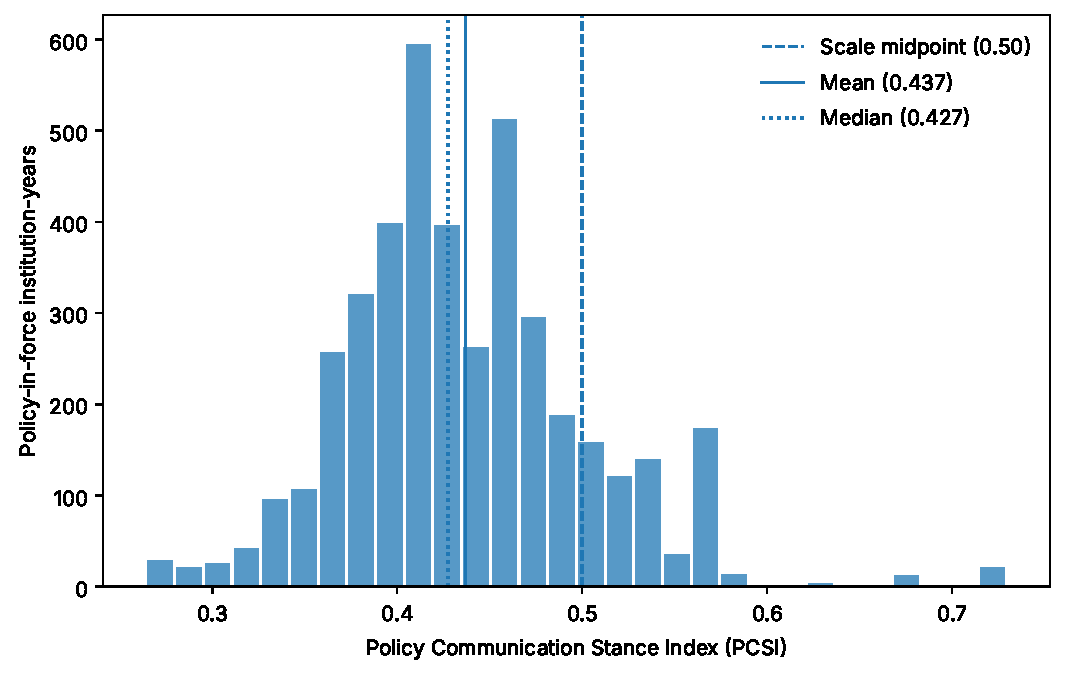
\includegraphics[width=0.82\textwidth]{fig1_pci_histogram.pdf}
\caption{Distribution of PCSI in the 1944--2025 policy-in-force panel ($N=4{,}277$). The dashed line marks the scale midpoint of 0.50; the solid and dotted lines mark the mean and median.}
\label{fig:hist}
\end{figure}

\subsection{Stance Has Become More Restrictive over Time}\label{sec:time}

We next examine how communicative stance has changed over time. Figure~\ref{fig:trend} shows the annual average PCSI from 1978, when the sample first includes at least five universities. The average reaches approximately 0.49 around 1980 and gradually declines to about 0.42 by 2025.

This decline could partly reflect changes in the universities represented in the dataset. We therefore examine changes within universities. Among the 93 universities represented by 2000, average PCSI falls from 0.447 to 0.422 by 2025. The estimated within-university trend is $-0.00112$ per year ($p=0.008$).\footnote{A within-university trend is estimated using university fixed effects, which account for stable differences between universities. Standard errors are clustered by university to allow observations from the same institution to be related. A standard error describes the precision of an estimate. The $p$-value measures how unusual an estimate at least this extreme would be under the statistical model if the true trend were zero.} Using only years with directly available policy text from 1980 onward produces a similar estimate of $-0.00117$ per year ($p=0.003$). Other fixed groups of universities also show negative trends (Appendix~\ref{app:temporal}, Table~\ref{tab:cohorts}).\footnote{A fixed group, or cohort, contains the universities already represented in the dataset by a chosen starting year. Following the same universities helps separate changes in their policy language from changes in the institutions covered by the archive.} The estimate based only on source texts from 2000 onward is negative but less precise (Appendix Table~\ref{tab:observed-trends}).

\begin{figure}[htbp]
\centering
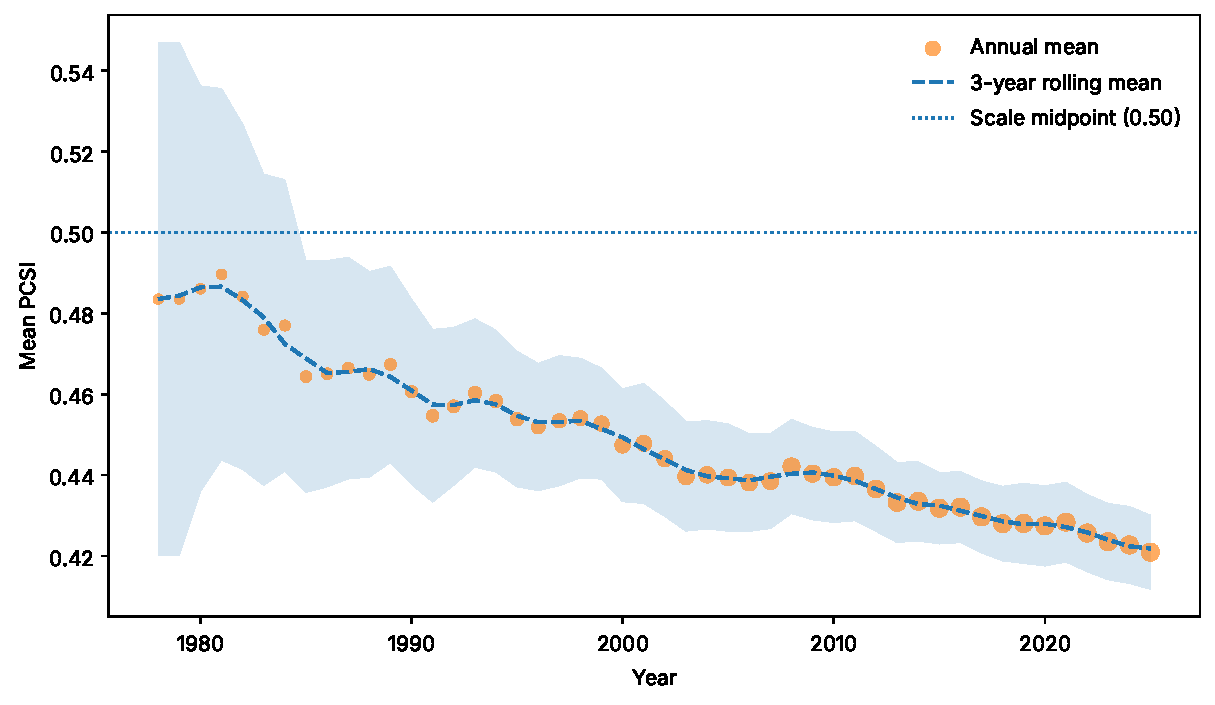
\includegraphics[width=0.86\textwidth]{fig3_temporal_trend_pcsi.pdf}
\caption{Annual mean PCSI, 1978--2025. Points show annual averages in the policy-in-force panel, with point size proportional to the number of universities. The shaded band shows the 95\% confidence interval, the dashed line shows a three-year rolling mean, and the dotted line marks the midpoint of 0.50. Years before 1978 are omitted because fewer than five universities are represented.}
\label{fig:trend}
\end{figure}

One possible explanation for this decline is that the underlying IP rules have changed. For example, the Supreme Court's decision in \emph{Stanford v.\ Roche} (2011) highlighted the legal importance of wording used to assign patent rights.\footnote{\emph{Board of Trustees of the Leland Stanford Junior University v.\ Roche Molecular Systems, Inc.}, 563 U.S. 776 (2011). The decision distinguished a promise to assign rights in the future from a present assignment of rights. It does not establish how widely universities subsequently revised their policies.} Such developments could influence the language of ownership and assignment provisions. We therefore examine whether the decline in PCSI is concentrated in these clauses or appears across other policy topics.

Figure~\ref{fig:topics} reports trends for different policy topics identified through keywords. Ownership and assignment language shows little change, with an estimated trend of $-0.0003$ per year ($p=0.64$). In contrast, disclosure, revenue-sharing, and administrative language show negative trends. The estimates for the remaining topics are also negative, although several are not statistically precise. These findings suggest that the overall decline is not confined to ownership and assignment provisions. Appendix Table~\ref{tab:topics} reports the estimates for each topic.

We also examine whether the decline reflects changes within policy topics or changes in the share of text devoted to different topics. For the 63 universities with policy text in both 1980--1999 and 2010--2025, average PCSI declined by 0.029. Changes within keyword-defined topics account for 77 percent of this decline, while changes in the mix of topics account for 23 percent.\footnote{We use a shift-share decomposition to separate changes in average scores within categories from changes in the relative shares of those categories. The calculation is performed separately for each university and then averaged across the 63 universities. Appendix~\ref{app:topics} provides the formula and additional details.} A similar analysis based on grammatical rule forms attributes 94 percent of the decline to changes within those forms (Appendix Table~\ref{tab:decomp}).

These results indicate that the changing composition of policy topics and rule forms explains only part of the decline in PCSI. Most of the change occurs within the categories we measure. However, because these categories are identified through keywords, changes within them may reflect differences in legal requirements as well as differences in how those requirements are expressed.

\begin{figure}[htbp]
\centering
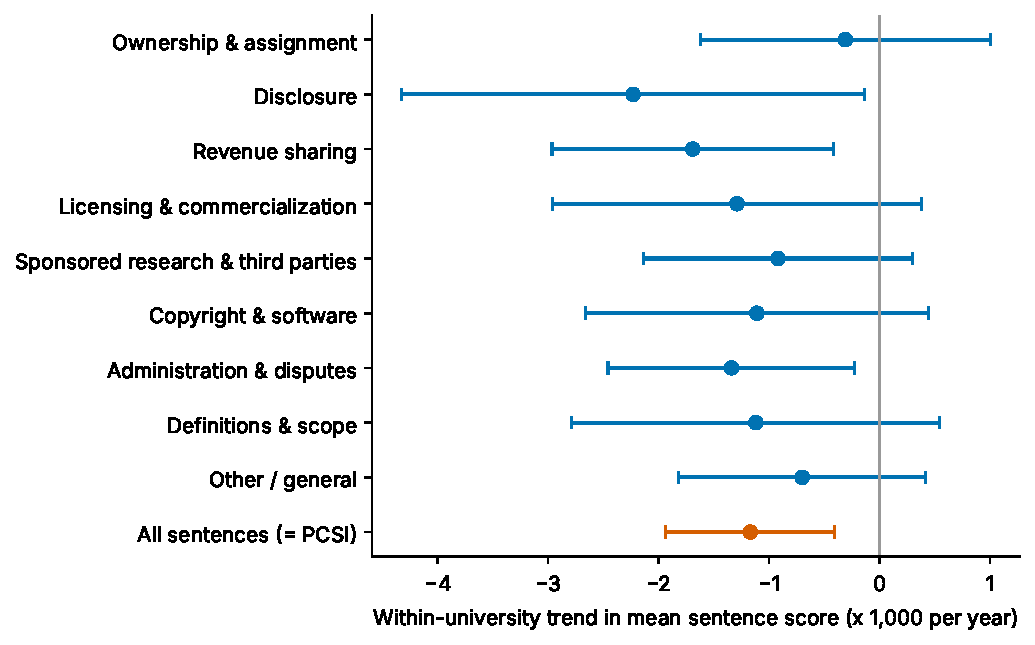
\includegraphics[width=0.82\textwidth]{fig_topic_trends.pdf}
\caption{Within-university trends in sentence stance by policy topic, 1980--2025. Points show annual trends estimated using years with directly available policy text; estimates are multiplied by 1,000. Bars show 95\% confidence intervals based on standard errors clustered by university. Topics are identified using keywords and may overlap (Appendix~\ref{app:topics}).}
\label{fig:topics}
\end{figure}

\subsection{Universities Differ Persistently in Stance}\label{sec:institutions}

Universities also differ in how they write their IP policies, and these differences tend to persist over time. In the annual panel, 61.0 percent of the variation in PCSI lies between universities, while 39.0 percent reflects changes within universities over time.\footnote{Between-university variation describes differences in universities' average PCSI scores. Within-university variation describes changes around each university's own average over time. The reported shares divide the total variation into these two components.} Carrying scores forward increases the measured persistence, but differences remain substantial when we consider only years with directly available policy text. In that sample, 48.7 percent of the variation lies between universities (Appendix Table~\ref{tab:variance}). Changes between successive policy revisions are generally modest, with a median absolute change of 0.021 across 330 revisions.\footnote{The absolute change is the size of the difference between two successive scores, regardless of whether the score increased or decreased. The median is the middle value after these changes are ordered.} These patterns suggest that universities maintain relatively stable differences in their policy language.

We next examine whether these differences are related to institutional characteristics. Table~\ref{tab:inst-means} reports average PCSI by university type. Private R1 universities have an average score of 0.456, compared with 0.427 for public R1 universities.\footnote{R1 is a Carnegie research classification indicating very high research activity in the historical classification system. The dataset records an R1 indicator but not the Carnegie edition used to construct it. Universities without the recorded R1 flag are therefore labeled ``non-R1'' rather than assumed to hold an official R2 designation.} Land-grant universities average 0.420, compared with 0.442 for other universities. Rank-based tests indicate differences across institutional types and between land-grant and other universities. Both comparisons remain statistically significant after adjusting for multiple testing. We find weaker evidence of differences by medical-school status or urbanicity (Appendix~\ref{app:inst}, Table~\ref{tab:holm}).\footnote{Rank-based tests compare groups using the ordering of observations rather than assuming normally distributed scores. We use Kruskal--Wallis and Wilcoxon tests. Because conducting several tests increases the chance of finding a statistically significant result by chance, we apply the Holm correction across four comparisons.}

\begin{table}[htbp]
\centering
\small
\caption{University-Level PCSI by Institutional Characteristics}
\label{tab:inst-means}
\begin{threeparttable}
\begin{tabular}{lcccc}
\toprule
Group & $N$ & Mean & SD & Range \\
\midrule
\multicolumn{5}{l}{\textit{Carnegie classification and control}} \\
\quad Private R1 & 38 & 0.456 & 0.046 & [0.337, 0.534] \\
\quad Public R1 & 86 & 0.427 & 0.051 & [0.328, 0.585] \\
\quad Private non-R1 & 8 & 0.406 & 0.053 & [0.342, 0.459] \\
\quad Public non-R1 & 18 & 0.441 & 0.058 & [0.376, 0.580] \\
\multicolumn{5}{l}{\textit{Mission and program}} \\
\quad Land-grant & 47 & 0.420 & 0.047 & [0.338, 0.585] \\
\quad Non-land-grant & 103 & 0.442 & 0.053 & [0.328, 0.580] \\
\quad Medical school & 118 & 0.438 & 0.053 & [0.328, 0.585] \\
\quad No medical school & 32 & 0.422 & 0.047 & [0.342, 0.519] \\
\multicolumn{5}{l}{\textit{Urbanicity}} \\
\quad Rural & 15 & 0.425 & 0.041 & [0.372, 0.519] \\
\quad Semi-urban & 48 & 0.422 & 0.047 & [0.338, 0.539] \\
\quad City & 82 & 0.443 & 0.057 & [0.328, 0.585] \\
\bottomrule
\end{tabular}
\begin{tablenotes}[flushleft]\footnotesize
\item \textit{Notes:} Unit of analysis is the university; PCSI is averaged across each university's policy-in-force years before group statistics are computed. Five universities lack urbanicity data. Rank-based tests are reported in Appendix~\ref{app:inst}.
\end{tablenotes}
\end{threeparttable}
\end{table}


Table~\ref{tab:inst-reg} examines these characteristics together. When we use one average score per university, the private-R1 difference decreases from 0.029 to approximately 0.020 after accounting for land-grant status, medical-school status, urbanicity, and region. The estimate is no longer statistically precise.\footnote{Regression coefficients describe differences associated with a characteristic after accounting for the other variables included in the model. An estimate is imprecise when its standard error is large relative to its size, making it difficult to distinguish the estimated association from zero. These coefficients do not establish causal effects.}

University averages may also reflect differences in when policies were written. To account for this, Column (4) uses university-years with directly available policy text and includes source-year fixed effects.\footnote{Source-year fixed effects account for differences associated with the calendar year in which the underlying policy document was written. This allows the regression to compare policies from the same year rather than mixing policies written in different periods.} The estimated private-R1 difference is 0.040 (standard error 0.012), while the land-grant coefficient falls to $-0.005$ and is not statistically distinguishable from zero.

\begin{table}[htbp]
\centering
\small
\caption{Institutional Correlates of PCSI}
\label{tab:inst-reg}
\begin{threeparttable}
\begin{tabular}{lcccc}
\toprule
 & \multicolumn{3}{c}{University means} & Source-text years \\
\cmidrule(lr){2-4}\cmidrule(lr){5-5}
 & (1) & (2) & (3) & (4) \\
\midrule
Private R1 & 0.029*** & 0.019 & 0.021 & 0.040*** \\
 & (0.009) & (0.012) & (0.014) & (0.012) \\
Private non-R1 & $-$0.021 & $-$0.031 & $-$0.035 & $-$0.006 \\
 & (0.021) & (0.023) & (0.023) & (0.018) \\
Public non-R1 & 0.014 & 0.007 & 0.011 & 0.005 \\
 & (0.015) & (0.020) & (0.018) & (0.011) \\
Land-grant &  & $-$0.014 & $-$0.011 & $-$0.005 \\
 &  & (0.012) & (0.013) & (0.012) \\
Medical school &  & 0.014 & 0.010 & 0.006 \\
 &  & (0.011) & (0.011) & (0.009) \\
\midrule
Urbanicity controls & No & Yes & Yes & Yes \\
Region fixed effects & No & No & Yes & Yes \\
Source-year fixed effects & No & No & No & Yes \\
$R^2$ & 0.074 & 0.111 & 0.161 & 0.291 \\
Observations & 150 & 145 & 144 & 452 \\
Universities & 150 & 145 & 144 & 144 \\
\bottomrule
\end{tabular}
\begin{tablenotes}[flushleft]\footnotesize
\item \textit{Notes:} Dependent variable is PCSI. Columns (1)--(3) use one observation per university (mean policy-in-force PCSI) with HC3 robust standard errors; Columns (2)--(3) omit universities with missing covariates. Column (4) uses university-years with directly available policy text, compares policies written in the same year through source-year fixed effects, and clusters standard errors by university. Public R1, rural, and Midwest are the omitted categories. *** $p<0.01$; ** $p<0.05$; * $p<0.10$.
\end{tablenotes}
\end{threeparttable}
\end{table}


The private-R1 difference is the clearest institutional pattern in these comparisons, although its statistical precision varies across specifications and weighting choices (Appendix Table~\ref{tab:inst-robust}). Overall, observable institutional characteristics explain only a modest share of the variation in average PCSI across universities. Broad institutional categories account for some differences in policy language, but much of the variation remains unexplained.

% =====================================================================

\section{Discussion}\label{sec:discussion}

Our findings show that university IP policies differ in how they express institutional authority, obligations, and support. The average PCSI is 0.437, and 86 percent of annual policy observations fall below the index midpoint. This indicates that restrictive language receives more emphasis than supportive language in most policies. However, restrictive does not necessarily mean negative or undesirable. Universities need rules governing invention disclosure, ownership, and licensing, and clear obligations can serve legitimate institutional purposes. Similarly, supportive language does not necessarily imply more generous rights or better treatment of inventors. PCSI measures how these rules are expressed, rather than whether the rules themselves are appropriate or beneficial.

The distinction between policy language and legal requirements is also supported by our measurement results. The grammatical forms of rules, including obligations, permissions, prohibitions, and sanctions, explain only 4.8 percent of the variation in sentence scores. An index that removes average differences across these forms remains closely correlated with PCSI ($r=0.94$). These findings suggest that communicative stance is not simply a count of mandatory rules. Research on organizational communication has long emphasized that formal documents convey institutional expectations alongside their explicit provisions \citep{cooren2004textual,fairhurst2004organizations}. Our analysis adds empirical evidence from university IP policies by showing that differences in supportive and restrictive language cannot be explained by basic grammatical rule forms alone. This does not mean that stance is independent of legal content, since our keyword measures cannot capture every aspect of a provision.

We also find that communicative stance differs persistently across universities. Even when we consider only years with directly available policy text, 48.7 percent of the variation in PCSI lies between universities. Private R1 universities tend to use more supportive language than public R1 universities, with an estimated difference of 0.040 in the specification comparing policies written in the same year. Yet observable institutional characteristics explain only a modest share of the differences in average PCSI. These results add another dimension to research on university technology transfer, which has emphasized differences in organizational practices, administrative arrangements, and interactions between faculty and technology-transfer offices (TTOs) \citep{jensen2003disclosure,siegel2003assessing,owensmith2001patent}. Our findings show that universities also differ in the language of the formal policies governing these activities. One possible reason for this persistence is that institutions retain wording from earlier documents and revise it gradually, as research on contractual language suggests \citep{kahan1997standardization,choi2013dynamics}. We cannot establish that this process explains the differences observed in our sample.

Another important finding is the gradual shift toward more restrictive language since 1980. The decline remains when we follow the same universities and when we use only years with directly available policy text. It also appears across several policy topics rather than being confined to ownership and assignment provisions. In the balanced sample, changes within keyword-defined topics account for 77 percent of the overall decline. These results suggest that the shift cannot be explained solely by changes in the types of provisions universities include in their policies. Research on institutional change suggests that organizations operating in the same field may respond to shared legal and professional pressures \citep{dimaggio1983iron,edelman1992legal}. Such pressures offer one possible explanation for the broader pattern we observe. However, our analysis does not identify the causes of the decline, and changes within policy topics may also reflect changes in legal requirements.

These findings raise a question for the literature on TTO governance. How might differences in written policy language relate to the institutional practices through which researchers experience IP rules? Studies have shown that faculty participation in technology transfer is influenced by interactions with TTO personnel, administrative procedures, and the local institutional environment \citep{owensmith2001patent,jensen2003disclosure,siegel2003assessing,bercovitz2008academic}. Our results identify variation in the written policies that provide a formal reference for these activities. Inventors do not necessarily need to read the policies directly for the documents to be relevant to institutional practice. TTO staff and administrators may draw on them when explaining disclosure requirements, interpreting ownership provisions, or guiding commercialization. Whether these interactions reflect the communicative stance of written policies remains unknown. PCSI offers a way to examine that relationship in future research, but our findings do not establish that policy language influences TTO behavior or inventor decisions.

The study also has limitations. The annual panel assumes that the most recent available policy remains in force until a newer document is found, although the main patterns remain when we use only years with directly available text. The classifier analyzes individual sentences and may miss meaning that depends on surrounding passages. The original human-coded training records are no longer available, so the historical model accuracy cannot be independently reassessed. Our measures of policy topics and rule forms also capture only part of the legal content. Finally, the analysis uses predicted sentence scores, and although alternative versions of PCSI produce similar findings (Appendix~\ref{app:uncertainty}), measurement uncertainty remains. These limitations reinforce the scope of our contribution: PCSI measures differences in written policy communication, not the quality of university governance or its effects on innovation.

% =====================================================================

\section{Conclusion}\label{sec:conclusion}

We introduce the Policy Communication Stance Index (PCSI) to examine how universities communicate intellectual-property rules, rather than focusing only on what those rules require. Our findings reveal systematic differences in written policy language across universities and over time, highlighting an aspect of IP governance that existing measures of institutional characteristics and formal policy provisions do not fully capture. These differences may be relevant to technology-transfer offices, which interpret and administer institutional rules in their interactions with researchers. Although we do not examine how written language influences these interactions, PCSI provides a foundation for doing so. By measuring how universities express authority, obligations, and support, we extend the study of university IP governance beyond formal rules to the language through which they are communicated.


\section*{Data and Code Availability}

The policy-sentence data, classifier scores, derived indices, replication code, and manuscript source are available at \url{https://github.com/krish533/PCSI}. The repository provides instructions for obtaining the classifier weights from the archived development project. The original human-coded training records are not available, so the historical classifier evaluation cannot be reproduced independently.

\singlespacing
\bibliographystyle{plainnat}
\bibliography{references}

% =====================================================================
\newpage
\appendix
\onehalfspacing
\renewcommand{\thetable}{\thesection\arabic{table}}
\renewcommand{\thefigure}{\thesection\arabic{figure}}

\section{Data Construction}\label{app:data}
\setcounter{table}{0}

Our analysis uses 87,159 cleaned sentences from 518 intellectual-property (IP) policy documents covering 150 U.S.\ research universities between 1944 and 2025. Each sentence is linked to its university, document year, and source file. The original archive contains one additional sentence from 1925, which falls outside the study period and is excluded from the analysis.

When a university has more than one relevant document in a year, we combine the sentences before constructing PCSI. This produces 480 university-years with directly available policy text. For subsequent years without a newer document, we carry the latest score forward until another policy appears. The resulting annual panel contains 4,277 university-year observations through 2025. Each observation retains the year of the source document, allowing us to distinguish directly observed policy texts from carried-forward scores.

For comparisons based on university averages, we calculate one average PCSI per university so that every institution counts once. Other analyses use the annual panel or only years with directly available policy text, as indicated in the relevant tables.

\section{Coding Rubric and Classifier}\label{app:model}
\setcounter{table}{0}

\paragraph{Coding rubric.}
The coding framework distinguishes supportive, neutral, and restrictive language. Supportive sentences emphasize assistance, guidance, encouragement, collaboration, or shared interests. Restrictive sentences emphasize mandatory assignment, institutional authority, prohibitions, sanctions, or compliance. Neutral sentences mainly define terms, describe arrangements, or explain procedures.

The original protocol assigned each sentence a label based on its main message. Several trained coders applied the rubric, and disagreements were resolved through adjudication. The categories describe how policy requirements are expressed. They do not indicate whether a legal provision is justified, generous, or effective.

\paragraph{Available training records.}
The original labeled sample contained 2,732 sentences, with 2,458 used for training and 274 held out for evaluation. The recorded evaluation results are 90.1 percent accuracy and a macro-F1 score of 0.894. The original labeled sentences and individual coder records were not preserved. We therefore cannot repeat the historical evaluation or calculate agreement among the original coders.

The replication package includes the model configuration, tokenizer, calibration parameter, and recorded evaluation metrics. The classifier weights are stored separately in the archived development repository, with retrieval instructions provided in the current repository.

\paragraph{Classifier and calibration.}
Table~\ref{tab:classifier} reports the classifier settings. For each sentence, the model assigns probabilities to the restrictive, neutral, and supportive categories. We apply temperature scaling before using these probabilities to construct sentence scores. This method adjusts the confidence of the predicted probabilities without changing the most likely category \citep{guo2017calibration}.

A reproducibility check used the saved classifier to rescore a random sample of 2,000 sentences. The recalculated probabilities differed from the stored values by no more than $4\times10^{-6}$, and the predicted labels matched for every sentence. Rebuilding the university-year indices from the stored sentence scores also reproduced the released indices exactly. These checks assess the scoring and aggregation procedures; they do not replace evaluation against the original human labels.

\begin{table}[htbp]
\centering
\small
\caption{Preserved Classifier Configuration}
\label{tab:classifier}
\begin{threeparttable}
\begin{tabular}{lr}
\toprule
Parameter & Value \\
\midrule
Base model & \texttt{bert-base-uncased} \\
Transformer layers & 12 \\
Attention heads & 12 \\
Hidden size & 768 \\
Intermediate size & 3,072 \\
Maximum input length & 256 tokens \\
Output classes & 3 \\
Training sentences & 2,458 \\
Validation sentences & 274 \\
Total labeled sentences & 2,732 \\
Temperature parameter & $T = 0.8462$ \\
Validation accuracy & 0.901 \\
Validation macro-F1 & 0.894 \\
\bottomrule
\end{tabular}
\begin{tablenotes}[flushleft]\footnotesize
\item \textit{Notes:} Configuration and metrics are read from the preserved model artifacts in the replication package.
\end{tablenotes}
\end{threeparttable}
\end{table}


\section{Aggregation and Persistence}\label{app:robust}
\setcounter{table}{0}

We examine whether PCSI depends on how sentence scores are combined. Table~\ref{tab:aggregation} compares the baseline mean with three alternatives: the median, a 5-percent trimmed mean, and a mean weighted by sentence length. We compare their scores, correlations, and rankings. We also report midpoint agreement, the share of observations that the baseline and an alternative place on the same side of 0.50.

Trimming produces almost identical scores to the baseline. Length weighting also gives similar results. The median changes levels more substantially but preserves much of the ranking across policies, with a rank correlation of 0.878.

\begin{table}[htbp]
\centering
\small
\caption{Sensitivity to Alternative Sentence Aggregation Rules}
\label{tab:aggregation}
\begin{threeparttable}
\begin{tabular}{lcccc}
\toprule
Aggregation & Mean & Pearson $r$ & Spearman $\rho$ & Midpoint agreement \\
\midrule
Baseline (unweighted mean) & 0.437 & 1.000 & 1.000 & 1.000 \\
Median PCSI & 0.471 & 0.623 & 0.878 & 0.937 \\
5\% trimmed mean & 0.431 & 0.999 & 1.000 & 1.000 \\
Length-weighted mean & 0.433 & 0.930 & 0.906 & 0.933 \\
\bottomrule
\end{tabular}
\begin{tablenotes}[flushleft]\footnotesize
\item \textit{Notes:} $N = 4{,}277$ policy-in-force university-years. Correlations are with baseline PCSI. Midpoint agreement is the share of observations that the baseline and the alternative place on the same side of 0.50.
\end{tablenotes}
\end{threeparttable}
\end{table}


Table~\ref{tab:variance} separates variation in PCSI into differences between universities and changes within universities over time. We report the shares for the baseline and alternative measures, using both the annual panel and the years with directly available policy text. Carrying scores forward increases measured persistence, but substantial differences between universities remain when we restrict the analysis to directly observed texts.

\begin{table}[htbp]
\centering
\small
\caption{Between- and Within-University Variation}
\label{tab:variance}
\begin{threeparttable}
\begin{tabular}{lcc}
\toprule
Specification & Between share & Within share \\
\midrule
\multicolumn{3}{l}{\textit{Policy-in-force panel}} \\
\quad Baseline & 0.610 & 0.390 \\
\quad Median & 0.434 & 0.566 \\
\quad Trimmed mean & 0.616 & 0.384 \\
\quad Length-weighted mean & 0.589 & 0.411 \\
\multicolumn{3}{l}{\textit{Years with source text}} \\
\quad Baseline & 0.487 & 0.513 \\
\quad Median & 0.300 & 0.700 \\
\quad Trimmed mean & 0.494 & 0.506 \\
\quad Length-weighted mean & 0.463 & 0.537 \\
\bottomrule
\end{tabular}
\begin{tablenotes}[flushleft]\footnotesize
\item \textit{Notes:} Shares partition the total sum of squared deviations of PCSI into between- and within-university components.
\end{tablenotes}
\end{threeparttable}
\end{table}


\section{Institutional Comparisons}\label{app:inst}
\setcounter{table}{0}

Table~\ref{tab:holm} reports rank-based comparisons across institutional characteristics, with Holm-adjusted $p$-values. The adjustment accounts for conducting four comparisons and reduces the risk of treating a chance difference as statistically significant.

The descriptive gaps are similar across alternative aggregation methods. The private-R1 minus public-R1 difference is 0.029 with the baseline index, 0.018 with the median, and 0.032 with the trimmed and length-weighted means. The land-grant gap ranges from $-0.020$ to $-0.024$. Using only years with directly available policy text, the two gaps are 0.033 and $-0.019$, respectively.

\begin{table}[htbp]
\centering
\small
\caption{Institutional Comparisons with Multiple-Testing Adjustment}
\label{tab:holm}
\begin{threeparttable}
\begin{tabular}{llcc}
\toprule
Characteristic & Test & Raw $p$ & Holm $p$ \\
\midrule
Carnegie classification and control & Kruskal--Wallis & 0.004 & 0.014 \\
Land-grant status & Wilcoxon rank-sum & 0.010 & 0.029 \\
Urbanicity & Kruskal--Wallis & 0.055 & 0.111 \\
Medical-school status & Wilcoxon rank-sum & 0.172 & 0.172 \\
\bottomrule
\end{tabular}
\begin{tablenotes}[flushleft]\footnotesize
\item \textit{Notes:} University-level mean PCSI ($N=150$; 145 for urbanicity). The Holm adjustment is applied to this family of four tests.
\end{tablenotes}
\end{threeparttable}
\end{table}


Table~\ref{tab:inst-robust} examines whether the regression results change across samples and weighting methods. Some specifications give greater weight to universities that contribute more documents or sentences. These comparisons show whether the reported institutional patterns depend heavily on those universities.

The timing of available policy documents also differs by university type. The average source-document year is 2002.3 for private R1 universities and 2005.1 for public R1 universities. Because PCSI changes over time, averages across universities may partly reflect when their documents were written. Column (4) of Table~\ref{tab:inst-reg} therefore includes source-year fixed effects, comparing policies from the same year. The private-R1 difference is larger in this specification. These estimates describe associations rather than causal effects of institutional type.

The R1 indicator comes from the institutional information supplied with the data. Its original Carnegie classification edition is not recorded. We therefore call universities without the R1 flag ``non-R1'' rather than assuming they hold an independently verified R2 designation.

\begin{table}[htbp]
\centering
\small
\caption{Private-R1 and Land-Grant Coefficients Across Samples and Estimators}
\label{tab:inst-robust}
\begin{threeparttable}
\begin{tabular}{lccccc}
\toprule
 & \multicolumn{2}{c}{Type only} & \multicolumn{3}{c}{Full controls} \\
\cmidrule(lr){2-3}\cmidrule(lr){4-6}
 & Private R1 & $N$ & Private R1 & Land-grant & $N$ \\
\midrule
University means & 0.029*** & 150 & 0.021 & $-$0.011 & 144 \\
 & (0.009) & & (0.014) & (0.013) & \\
WLS, weight = source policy years & 0.027** & 144 & 0.020 & $-$0.021 & 144 \\
 & (0.010) & & (0.015) & (0.015) & \\
WLS, weight = sentences & 0.021 & 144 & 0.023 & 0.005 & 144 \\
 & (0.014) & & (0.023) & (0.028) & \\
Era-adjusted university means & 0.029*** & 144 & 0.022 & $-$0.009 & 144 \\
 & (0.009) & & (0.014) & (0.013) & \\
Source-text years, year FE & 0.040*** & 452 & 0.040*** & $-$0.005 & 452 \\
 & (0.010) & & (0.012) & (0.012) & \\
Source-text years from 1980, year FE & 0.039*** & 439 & 0.038*** & $-$0.005 & 439 \\
 & (0.010) & & (0.012) & (0.012) & \\
\bottomrule
\end{tabular}
\begin{tablenotes}[flushleft]\footnotesize
\item \textit{Notes:} Dependent variable is PCSI; public R1 is the omitted type. ``Full controls'' adds land-grant, medical-school, and urbanicity indicators and region fixed effects; it uses the 144 universities with complete covariates. Re-estimating the type-only specification on those same 144 universities gives a private-R1 coefficient of 0.029*** (0.009), so the change between the two columns is not due to the smaller sample. University-mean rows use HC3 standard errors. Era-adjusted means subtract each calendar year's cross-sectional mean from the policy-in-force panel before averaging within university. Source-text rows use university-years with directly available policy text, include source-year fixed effects, and cluster standard errors by university. *** $p<0.01$; ** $p<0.05$; * $p<0.10$.
\end{tablenotes}
\end{threeparttable}
\end{table}


\section{Word-Based Diagnostics}\label{app:linguistic}
\setcounter{table}{0}

We construct three word-based measures to help interpret PCSI: Tone, Clarity, and Legal Load. These measures summarize selected features of the written policies. They are not independent measures of communicative stance or direct evidence of how readers interpret the documents.

Tone combines supportive and collaborative language with indicators of obligations, control, and sanctions. Clarity combines sentence length with procedural language. Legal Load captures legal and IP-related vocabulary. We first standardize each component by subtracting its mean and dividing by its standard deviation. We then combine the standardized components as follows:

\begin{align}
\text{Tone}
&= \tfrac{1}{6}\big[
 z(\text{supportive}) + z(\text{second person}) + z(\text{inclusive we}) \notag\\
&\qquad - z(\text{restrictive}) - z(\text{sanction}) - z(\text{obligation modal share})\big],\\
\text{Clarity}
&= \tfrac{1}{3}\big[-z(\text{mean sentence length}) - z(\text{long-sentence share}) + z(\text{procedural share})\big],\\
\text{Legal Load}
&= \tfrac{1}{2}\big[z(\text{legalese}) + z(\text{IP technical})\big].
\end{align}

Here, $z(\cdot)$ indicates a standardized variable. The supportive, restrictive, sanction, procedural, legalese, and IP-technical components come from word lists supplied in the replication code. Second-person language identifies direct forms of address, while inclusive ``we'' identifies collective forms of address.

The diagnostics capture different features of the text. Tone and Clarity correlate at 0.143, Tone and Legal Load at 0.029, and Clarity and Legal Load at $-0.296$. Table~\ref{tab:length} also examines whether policy length affects these relationships. The association between Tone and PCSI changes little after accounting for length. In the 480 years with directly available policy text, the three-diagnostic regression gives coefficients of 0.038 for Tone, 0.013 for Clarity, and 0.012 for Legal Load, with $R^2=0.151$.

\begin{table}[htbp]
\centering
\small
\caption{Linguistic Decomposition with Policy-Length Controls}
\label{tab:length}
\begin{threeparttable}
\begin{tabular}{lccc}
\toprule
 & Baseline & + Log words & + Log sentences \\
\midrule
Tone Index & 0.062*** & 0.059*** & 0.059*** \\
 & (0.012) & (0.012) & (0.012) \\
Clarity Index & 0.006 & 0.006 & 0.008 \\
 & (0.008) & (0.008) & (0.009) \\
Legal Load Index & 0.013** & 0.010 & 0.010 \\
 & (0.006) & (0.007) & (0.007) \\
\midrule
Policy-length control & No & Log words & Log sentences \\
$R^2$ & 0.236 & 0.244 & 0.241 \\
Observations & 4,277 & 4,277 & 4,277 \\
\bottomrule
\end{tabular}
\begin{tablenotes}[flushleft]\footnotesize
\item \textit{Notes:} University-clustered standard errors in parentheses. *** $p<0.01$; ** $p<0.05$; * $p<0.10$.
\end{tablenotes}
\end{threeparttable}
\end{table}


\section{Trends over Time}\label{app:temporal}
\setcounter{table}{0}

The composition of the archive changes over time as more universities enter the sample. To assess how this affects the estimated trend, we follow fixed groups of universities from several starting years. Table~\ref{tab:cohorts} reports these comparisons.

Every group has a lower average PCSI in 2025 than at its starting point, and every estimated within-university trend is negative. This suggests that the overall decline does not arise solely because different universities enter the archive at different times.

\begin{table}[htbp]
\centering
\small
\caption{PCSI Trends Within Fixed University Cohorts}
\label{tab:cohorts}
\begin{threeparttable}
\begin{tabular}{cccccc}
\toprule
Cohort start & Universities & Start mean & 2025 mean & FE trend per year & $p$ \\
\midrule
1990 & 34 & 0.461 & 0.421 & $-$0.00109 & 0.019 \\
1995 & 53 & 0.454 & 0.422 & $-$0.00131 & 0.002 \\
2000 & 93 & 0.447 & 0.422 & $-$0.00112 & 0.008 \\
2005 & 114 & 0.439 & 0.420 & $-$0.00103 & 0.011 \\
\bottomrule
\end{tabular}
\begin{tablenotes}[flushleft]\footnotesize
\item \textit{Notes:} Each cohort contains the universities already represented in the policy-in-force panel by the start year. Trends come from regressions of PCSI on year with university fixed effects; standard errors are clustered by university.
\end{tablenotes}
\end{threeparttable}
\end{table}


Table~\ref{tab:observed-trends} reports trends estimated using only years with directly available policy text. We estimate both a pooled trend and a within-university trend. The estimate based on texts from 2000 onward is negative but less precise.

We also examine whether the 2025 results depend heavily on older policy documents. Among the 70 universities whose latest available policy is no more than five years old, 91 percent have PCSI below the midpoint. The corresponding share is 92 percent among all 150 universities in the 2025 panel. Thus, the predominance of scores below 0.50 is also present among universities with relatively recent source documents.

\begin{table}[htbp]
\centering
\small
\caption{Temporal Trends Using Only Years with Source Policy Text}
\label{tab:observed-trends}
\begin{threeparttable}
\begin{tabular}{cccccc}
\toprule
Start year & $N$ & Pooled trend & FE trend & SE & $p$ \\
\midrule
1980 & 467 & $-$0.00115 & $-$0.00117 & (0.00039) & 0.003 \\
1990 & 443 & $-$0.00121 & $-$0.00128 & (0.00053) & 0.016 \\
2000 & 367 & $-$0.00109 & $-$0.00150 & (0.00093) & 0.105 \\
\bottomrule
\end{tabular}
\begin{tablenotes}[flushleft]\footnotesize
\item \textit{Notes:} University-years with directly available policy text from the start year onward. Standard errors are clustered by university.
\end{tablenotes}
\end{threeparttable}
\end{table}


\section{Clause Topics and Rule Forms}\label{app:topics}
\setcounter{table}{0}

\paragraph{Clause topics.}
We use keywords to identify eight broad topics in the policy texts: ownership and assignment, disclosure, revenue sharing, licensing and commercialization, sponsored research and third parties, copyright and software, administration and disputes, and definitions and scope. The keywords are:

\begin{itemize}
\item Ownership and assignment: \emph{assign}, \emph{ownership}, \emph{title}, \emph{vest}, \emph{belong}.
\item Disclosure: \emph{disclos}, \emph{invention report}.
\item Revenue sharing: \emph{royalt}, \emph{revenue}, \emph{net income/proceeds}, \emph{distribut}, \emph{equity}.
\item Licensing and commercialization: \emph{licens}, \emph{commerciali}, \emph{technology transfer}, \emph{start-up}, \emph{patent application}.
\item Sponsored research and third parties: \emph{sponsor}, \emph{grant}, \emph{federal}, \emph{government}, \emph{contract}, \emph{third part}.
\item Copyright and software: \emph{copyright}, \emph{software}, \emph{courseware}, \emph{scholarly work}.
\item Administration and disputes: \emph{appeal}, \emph{dispute}, \emph{committee}, \emph{review}, \emph{waive}, \emph{grievance}, \emph{amend}.
\item Definitions and scope: \emph{means}, \emph{defined}, \emph{applies to}, \emph{purpose}, \emph{scope}.
\end{itemize}

For the topic-specific trends, a sentence may belong to more than one topic. For the decomposition below, we assign each sentence to one main topic using the first matching category in the order listed above. Sentences without a match enter an ``other'' category.

Among sentences from 1980 onward, 59 percent match at least one topic. Ownership and assignment sentences have the lowest average score (0.335). Definitions and revenue-sharing sentences have higher averages, at 0.448 and 0.453, respectively. Table~\ref{tab:topics} reports the topic trends. These categories identify broad subjects, not the full legal meaning of each sentence.

\begin{table}[htbp]
\centering
\small
\caption{Within-University Trends in Sentence Stance by Clause Topic, 1980--2025}
\label{tab:topics}
\begin{threeparttable}
\begin{tabular}{lccccc}
\toprule
Topic & Share & Mean score & FE trend per year & SE & $p$ \\
\midrule
Ownership \& assignment & 0.142 & 0.335 & $-$0.00031 & (0.00067) & 0.644 \\
Disclosure & 0.057 & 0.357 & $-$0.00223 & (0.00107) & 0.037 \\
Revenue sharing & 0.131 & 0.453 & $-$0.00169 & (0.00065) & 0.010 \\
Licensing \& commercialization & 0.133 & 0.432 & $-$0.00129 & (0.00085) & 0.129 \\
Sponsored research \& third parties & 0.131 & 0.341 & $-$0.00092 & (0.00062) & 0.140 \\
Copyright \& software & 0.092 & 0.412 & $-$0.00111 & (0.00079) & 0.159 \\
Administration \& disputes & 0.141 & 0.425 & $-$0.00134 & (0.00057) & 0.018 \\
Definitions \& scope & 0.083 & 0.448 & $-$0.00112 & (0.00085) & 0.185 \\
Other / general & 0.409 & 0.427 & $-$0.00070 & (0.00057) & 0.213 \\
\midrule
All sentences (= PCSI) & 1.000 &  & $-$0.00117 & (0.00039) & 0.002 \\
\bottomrule
\end{tabular}
\begin{tablenotes}[flushleft]\footnotesize
\item \textit{Notes:} Each row regresses the university-year mean sentence score within a topic on year and university fixed effects, using source-text university-years from 1980 and universities observed in at least two such years; standard errors are clustered by university. Topics are assigned by keyword rules and can overlap; share is the fraction of 1980--2025 sentences matching the topic. Within-topic trends allow overlapping keyword matches. The exact shift-share calculation instead uses mutually exclusive primary topics and is reported separately in Table~\ref{tab:decomp}.
\end{tablenotes}
\end{threeparttable}
\end{table}


\paragraph{Decomposition.}
We examine whether changes in PCSI come from changes in average scores within topics or changes in the share of text devoted to each topic. We compare 1980--1999 with 2010--2025 for the 63 universities with directly available policy text in both periods. The two periods contain 8,353 and 28,175 sentences, respectively.

For university $i$ in period $t\in\{0,1\}$, let $s_{ikt}$ be the share of sentences in category $k$, and let $m_{ikt}$ be the category's average score. The university's mean score is

\begin{equation}
M_{it}=\sum_k s_{ikt}m_{ikt}.
\end{equation}

We divide the change between periods into two parts:

\begin{equation}
\begin{split}
M_{i1}-M_{i0}
&=\underbrace{\sum_k\frac{s_{ik1}+s_{ik0}}{2}(m_{ik1}-m_{ik0})}_{\text{Within-category change}}\\
&\quad+\underbrace{\sum_k\frac{m_{ik1}+m_{ik0}}{2}(s_{ik1}-s_{ik0})}_{\text{Composition change}}.
\end{split}
\end{equation}

The first part captures changes in average sentence scores within categories. The second captures changes in how much text belongs to each category. We calculate these contributions separately for each university and then average them, giving each university equal weight.

If a category appears in only one period for a university, we use its observed mean for both periods. This assigns the effect of the category's appearance or disappearance to composition. With this convention, the two components sum exactly to the observed change.

We repeat the exercise using grammatical rule forms instead of policy topics. These are two alternative descriptions of the same change and should not be added together. Table~\ref{tab:decomp} reports the results. Because topic and rule-form categories are based on keywords, within-category changes cannot be interpreted as changes in wording while legal requirements remain unchanged.

\begin{table}[htbp]
\centering
\small
\caption{Exact Shift--Share Decompositions of the Modern PCSI Decline}
\label{tab:decomp}
\begin{threeparttable}
\begin{tabular}{lrr}
\toprule
 & Exclusive primary topic & Deontic $\times$ sanction \\
\midrule
Early period: mean score (1980--1999) & 0.455454 & 0.455454 \\
Late period: mean score (2010--2025) & 0.426638 & 0.426638 \\
\textbf{Observed change} & \textbf{$-0.028816$} & \textbf{$-0.028816$} \\
Within-category contribution & $-0.022229$ & $-0.027077$ \\
Composition contribution & $-0.006587$ & $-0.001739$ \\
Within-category share of decline & 77.1\% & 94.0\% \\
Composition share of decline & 22.9\% & 6.0\% \\
Universities with policies in both periods & 63 & 63 \\
Early and late sentences & 8,353; 28,175 & 8,353; 28,175 \\
\bottomrule
\end{tabular}
\begin{tablenotes}[flushleft]\footnotesize
\item \textit{Notes:} The unit of comparison is a university appearing in both periods; universities are weighted equally. Each sentence is assigned to one primary topic by fixed keyword priority, or to one of eight deontic-by-sanction cells. Category changes are decomposed within each university using midpoint shares and midpoint conditional means, then averaged. If a category is absent in a period, its conditional mean is imputed from the observed period, assigning category entry/exit to composition. The university-level accounting identity holds to machine precision. These alternative decompositions are not additive and are sensitive to the coding rules and missing-category convention. The numbers are descriptive, not causal estimates.
\end{tablenotes}
\end{threeparttable}
\end{table}


\paragraph{Rule forms.}
We also use keywords to identify whether a sentence expresses an obligation, permission, or prohibition. These words are sometimes called \emph{deontic operators}. Each sentence receives one category, in the following order of priority:

\begin{itemize}
\item Prohibition: negated forms of \emph{shall}, \emph{must}, \emph{may}, \emph{will}, or \emph{can}, together with \emph{cannot}, \emph{prohibit}, and \emph{not permitted}.
\item Obligation: \emph{shall}, \emph{must}, \emph{is required}, \emph{requires}, \emph{obligat-}, \emph{agrees to}, and \emph{is expected to}.
\item Permission: \emph{may}, \emph{permit}, \emph{entitled}, \emph{discretion}, \emph{can}, and \emph{allow}.
\item None: sentences without a matching operator.
\end{itemize}

Sanction language is identified separately using terms such as \emph{violat-}, \emph{disciplin-}, \emph{sanction}, \emph{forfeit}, \emph{terminat-}, \emph{breach}, \emph{penalt-}, \emph{dismiss}, and \emph{revok-}.

Table~\ref{tab:rule-form} reports sentence scores by rule form. At the policy level, the shares of sentences expressing obligations, prohibitions, permissions, and sanctions explain 11 percent of the variation in PCSI across the 480 years with directly available text. This policy-level comparison is different from the sentence-level exercise reported in Section~\ref{sec:captures}. Keyword categories provide a simple comparison of grammatical forms, but they are not a complete legal interpretation of the provisions.

\begin{table}[htbp]
\centering
\small
\caption{Communicative Stance by Rule Form}
\label{tab:rule-form}
\begin{threeparttable}
\begin{tabular}{lcccc}
\toprule
Rule form & Share & Mean score & Restrictive & Supportive \\
\midrule
Obligation & 0.314 & 0.329 & 0.466 & 0.105 \\
Prohibition & 0.072 & 0.430 & 0.470 & 0.316 \\
Permission & 0.138 & 0.431 & 0.406 & 0.246 \\
No deontic operator & 0.475 & 0.467 & 0.226 & 0.160 \\
\midrule
Sanction language (any form) & 0.037 & 0.334 & 0.487 & 0.124 \\
\bottomrule
\end{tabular}
\begin{tablenotes}[flushleft]\footnotesize
\item \textit{Notes:} Deontic operators follow the Institutional Grammar of \citet{crawford1995grammar} and are assigned by keyword rules with priority prohibition $>$ obligation $>$ permission (Appendix~\ref{app:topics}). Sanction language (the grammar's ``or else'' component) can co-occur with any form. Restrictive and supportive shares use the classifier's most likely label. Rule form explains 4.8 percent of sentence-level variance in stance. The exact 63-university within-cell and composition changes are reported in Table~\ref{tab:decomp}.
\end{tablenotes}
\end{threeparttable}
\end{table}


\section{Alternative Versions of PCSI}\label{app:uncertainty}
\setcounter{table}{0}

The baseline PCSI uses predicted probabilities rather than only the most likely label for each sentence. It therefore retains information about the classifier's confidence. However, the regressions treat predicted scores as data and do not formally adjust their standard errors for classification uncertainty \citep{egami2023using,battaglia2024inference}.

We examine the sensitivity of our findings using three alternative versions of the index. First, we assign each sentence a score of 0, 0.5, or 1 based on its most likely predicted category. Second, we restrict the analysis to sentences for which the classifier assigns a probability of at least 0.90 to its most likely category, retaining about 66 percent of sentences. Third, we construct an index that removes average differences associated with grammatical rule forms.

Table~\ref{tab:alternatives} compares the main findings across these versions. In every case, most policies fall below the midpoint, approximately half of the variation in directly observed policy years lies between universities, and the within-university trend is negative. The private-R1 coefficient is also positive and statistically significant across the reported specifications.

We further examine whether the classifier's confidence changes over time. From the 1970s onward, the average probability assigned to the most likely category lies between 0.874 and 0.886 in every decade. These comparisons suggest that the main patterns do not depend on a single way of using the classifier's predictions. They do not, however, eliminate possible classification errors or provide a formal correction for model uncertainty.

\begin{table}[htbp]
\centering
\footnotesize
\caption{Headline Results Under Alternative Constructions of PCSI}
\label{tab:alternatives}
\begin{threeparttable}
\begin{tabular}{lcccccc}
\toprule
 & $r$ with & & Share & Between & FE trend, & \\
Construction & baseline & Mean & $<0.50$ & share & 1980+ & Private R1 \\
\midrule
Baseline PCSI &  & 0.429 & 0.896 & 0.487 & $-$0.00117*** & 0.040*** \\
 & & & & & (0.00039) & (0.012) \\
Hard labels & 0.980 & 0.425 & 0.856 & 0.487 & $-$0.00139*** & 0.042*** \\
 & & & & & (0.00044) & (0.013) \\
High-confidence sentences & 0.952 & 0.418 & 0.875 & 0.495 & $-$0.00134*** & 0.049*** \\
 & & & & & (0.00051) & (0.014) \\
Framing net of rule form & 0.943 & 0.427 & 0.894 & 0.492 & $-$0.00135*** & 0.032** \\
 & & & & & (0.00037) & (0.013) \\
\bottomrule
\end{tabular}
\begin{tablenotes}[flushleft]\footnotesize
\item \textit{Notes:} All columns use the 480 university-years with directly available policy text. Hard labels score each sentence 0, 0.5, or 1 by its most likely class. High-confidence uses only sentences whose largest calibrated class probability is at least 0.9 (about two-thirds of sentences). Framing net of rule form subtracts the mean score of each sentence's deontic-by-sanction cell before aggregation. The trend is the coefficient on year with university fixed effects, using universities with at least two source-text years from 1980; the private-R1 coefficient is from the Column (4) specification of Table~\ref{tab:inst-reg}. Standard errors clustered by university. *** $p<0.01$; ** $p<0.05$; * $p<0.10$.
\end{tablenotes}
\end{threeparttable}
\end{table}



\end{document}
